\documentclass[10pt]{article}
\usepackage[margin=0.7in]{geometry}
\usepackage{graphicx}
\usepackage{booktabs}
\usepackage{amsmath}
\begin{document}
\begin{center}
{\Large N53 K220 S3 root batching: valid run record}\par
2026-10-12 17:37 UTC; 27 frozen cells; run 20261012T1737Z
\end{center}
\noindent\textbf{Identity and host.} Curve EC1N53Ce0hb097de99be9a,
prime subgroup 21,044,858,204,113; K220 fixed 23,320-point base.
Three public Q, three rank seeds per Q, three strong-rho seeds.
Source and binary hashes: \texttt{../../FROZEN.json}.
Apple M4 Pro, macOS 26.6, Rust 1.93.1 release; shared-host L0.

\smallskip
\noindent\textbf{Execution and correctness.} All 27 process statuses are
\texttt{COMPLETED} within the 90-second and 16-GiB caps. Native analysis
and independent replay verified all nine control/candidate pairs:
rank 220/220, 220 accepted independent relations per IC arm,
same selected rank trace, base dump, root table, consumed root count,
target witness and scalar. The 9 rho arms verified the same public Q.
Raw records: \texttt{../../runs/}; native analysis:
\texttt{../../ANALYSIS.json}; native aggregate:
\texttt{../../RESULT\_DATA.json}.

\begin{center}
\begin{tabular}{lrr}
\toprule
Same-Q ratio, in-process ms & Median & Target-block 95\% interval\\
\midrule
Batch/control, cold IC & 0.737998 & [0.714128, 0.750321]\\
Batch/control, target online & 0.611643 & [0.568613, 0.903106]\\
Control/strong rho, cold & 78.145833 & [44.219726, 92.601592]\\
Batch/strong rho, cold & 52.585601 & [33.179008, 64.667877]\\
Control/strong rho, online & 0.489747 & [0.167802, 0.763394]\\
Batch/strong rho, online & 0.377771 & [0.102635, 0.442294]\\
\bottomrule
\end{tabular}
\end{center}
\noindent The intervals are 10,000 deterministic resamples of three target
blocks, retaining each block's three rank seeds. These are descriptive
timing summaries, without host-isolation admission or common-operation
\(S\) calibration. Source-level rank-root totals over nine cells:
80,790,012 versus 763,167 inversions; 1,211,850,180 versus
902,063,394 multiplication calls; 242,370,036 versus 39,684,684
squaring calls (control versus batch).

\clearpage
\begin{center}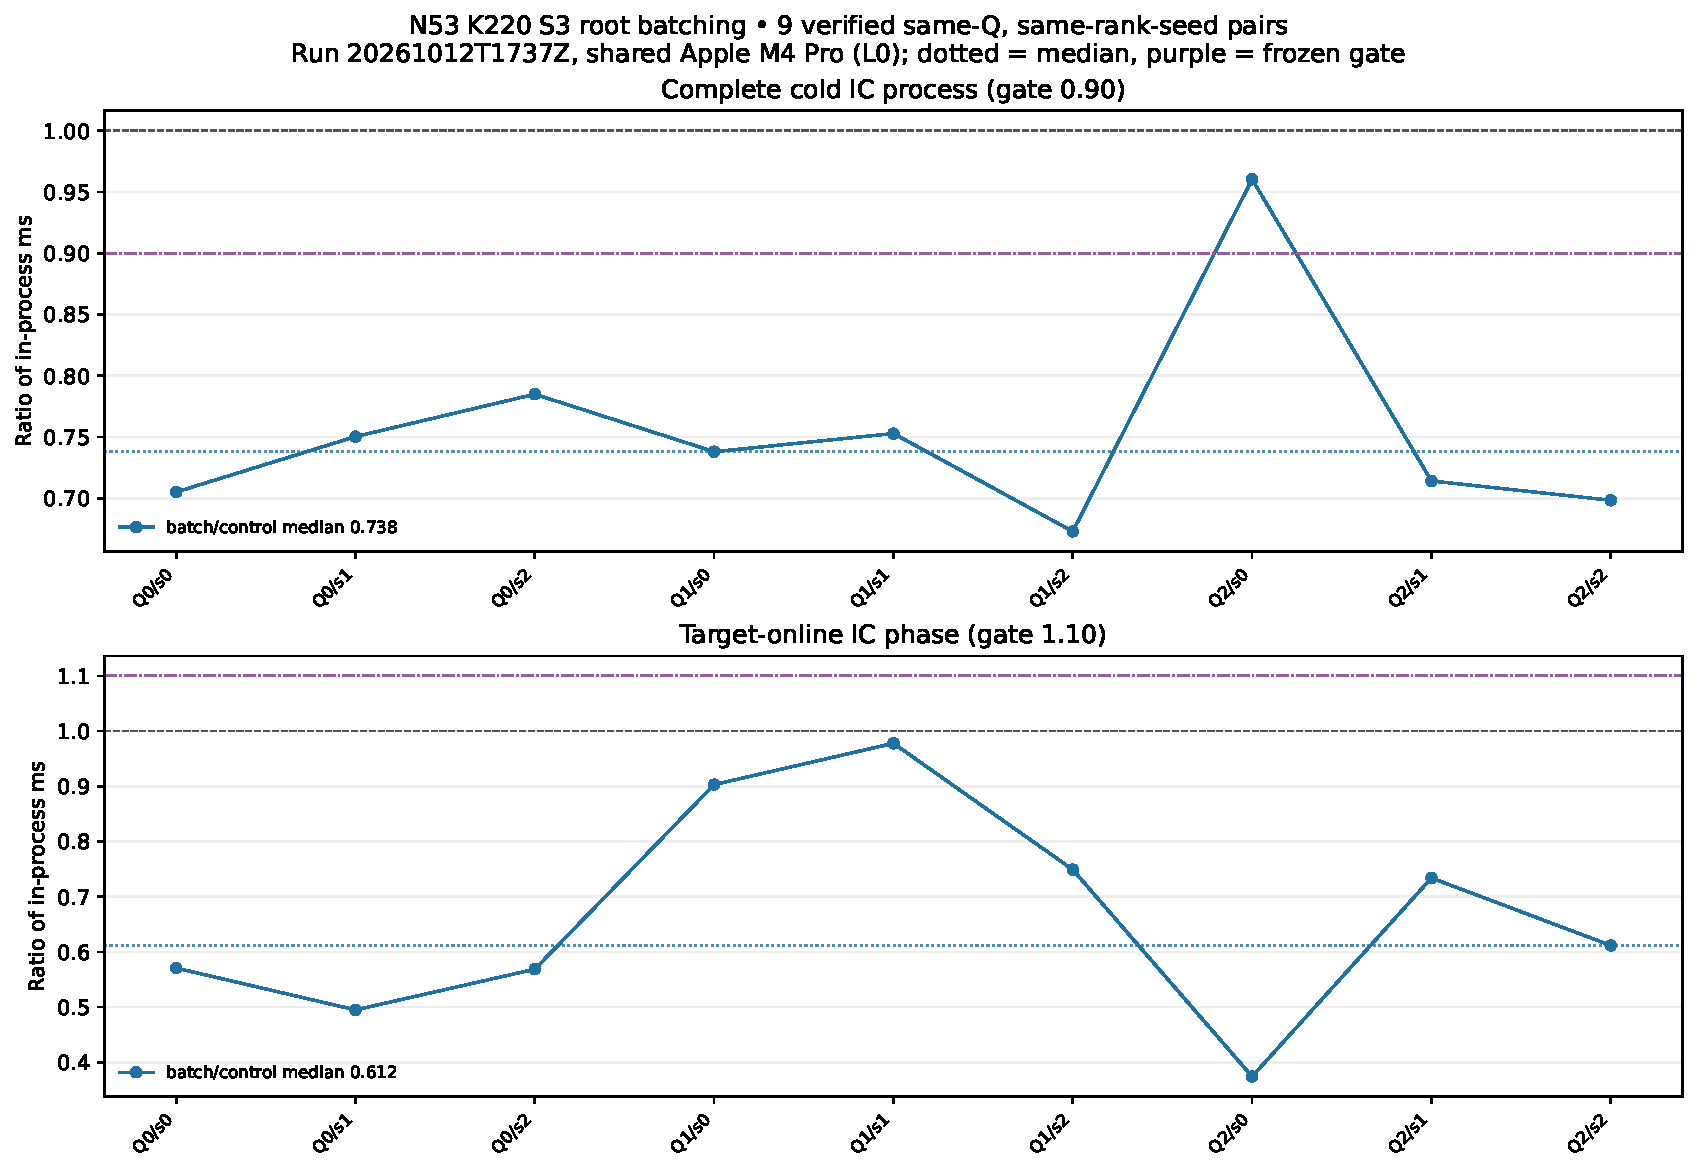
\includegraphics[width=\linewidth]{paired_ratios.pdf}\end{center}
\clearpage
\begin{center}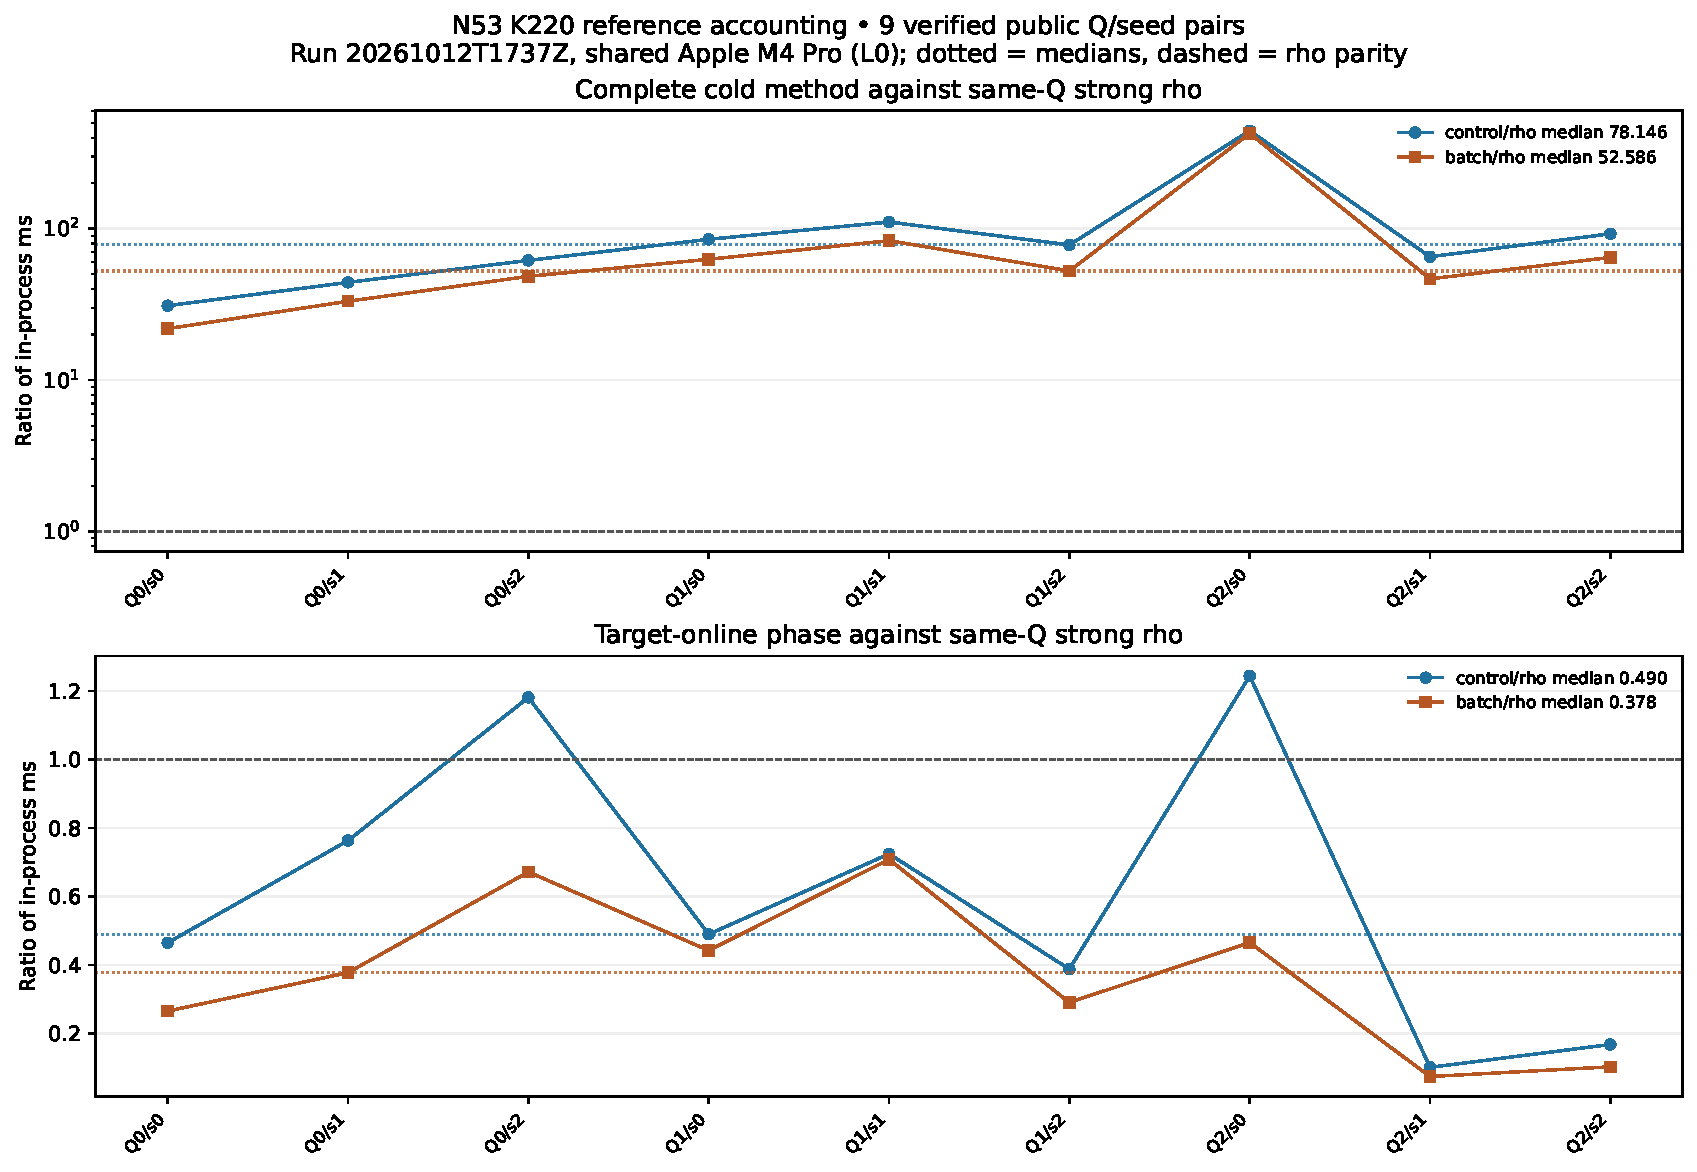
\includegraphics[width=\linewidth]{rho_reference.pdf}\end{center}
\end{document}
